%% LaTeX-Beamer template for KIT design
%% by Erik Burger, Christian Hammer
%% title picture by Klaus Krogmann
%%
%% version 2.1
%%
%% mostly compatible to KIT corporate design v2.0
%% http://intranet.kit.edu/gestaltungsrichtlinien.php
%%
%% Problems, bugs and comments to
%% burger@kit.edu

\documentclass[18pt]{beamer}

%% SLIDE FORMAT

% use 'beamerthemekit' for standard 4:3 ratio
% for widescreen slides (16:9), use 'beamerthemekitwide'

\usepackage{./templates/beamerthemekit}
% \usepackage{templates/beamerthemekitwide}


%\titleimage{mypicture}



\title[KDE and MSC]{Kernel Density Estimates and Mean Shift Clustering}
% \subtitle{Sommersemester 2018}
\author{Jonas Spinner}
\date{February 4, 2019}

\institute{Analytics and Statistics at the Institute of Operations Research}

% Bibliography

\usepackage{natbib}

%\usepackage[citestyle=authoryear,bibstyle=numeric,hyperref,backend=biber]{biblatex}
%\addbibresource{../latex/KDEaMSC.bib}
%\bibhang1em


%\usepackage{tikz}

%\usepackage{algorithm}
%\usepackage{algorithmic}

\usepackage{algpseudocode}
\usepackage{algorithm}
% keine "End"-Statements in Algorithmen
\algtext*{EndWhile}
\algtext*{EndIf}
\algtext*{EndFor}
\algtext*{EndProcedure}


\usepackage[utf8]{inputenc}
\usepackage[english]{babel}
\usepackage[T1]{fontenc}
\usepackage{amsmath,amsmath,lmodern}
\usepackage{bm}
\usepackage{bbm}

\usepackage{graphicx}
\usepackage{subfig}


\newcommand{\norm}[1]{\left\lVert#1\right\rVert}



\begin{document}

% change the following line to "ngerman" for German style date and logos
% \selectlanguage{ngerman}

%title page
\begin{frame}
\titlepage
\end{frame}

%table of contents
\begin{frame}{Outline}
	\tableofcontents
\end{frame}


\section{Introduction}
\begin{frame}{History}
	\begin{itemize}
		\item \cite{Fukunaga.1975}
		\item \cite{Comaniciu.2002}
		\item \cite{Comaniciu.2003}
	\end{itemize}
\end{frame}


\section{Kernel Density Estimates}
\begin{frame}
	\begin{align*}
		\hat{f}(\bm{x}) = \frac{1}{n h^d} \sum_{i=1}^{n} K\left(\frac{\bm{x} - \bm{x}_i}{h} \right)
	\end{align*}
	\[ \hat{f}(\bm{x}) = \frac{1}{n h^d} \sum_{i=1}^{n} K\left(\frac{\bm{x} - \bm{x}_i}{h} \right) \]
\end{frame}


\begin{frame}{Locally Weighted Mean}
	Weighted mean
	\begin{align*}
		\bm{\mu}^* = \frac{\sum_{i=1}^n \bm{x}_i w_i}{\sum_{i=1}^n w_i}
	\end{align*}
	
	With weights as a function around a point
	\begin{align*}
		w_i = w_{\bm{x}}(\bm{x}_i) = g\left(\norm{\frac{\bm{x} - \bm{x}_i}{h}}^2 \right)\\
		\bm{\mu}_h^*(\bm{x}) = \frac{\sum_{i=1}^n \bm{x}_i g\left(\norm{\frac{\bm{x} - \bm{x}_i}{h}}^2 \right)}{\sum_{i=1}^n g\left(\norm{\frac{\bm{x} - \bm{x}_i}{h}}^2 \right)}
	\end{align*}
\end{frame}


\section{Mean Shift Clustering}


\begin{frame}
	\begin{align*}
		\bm{x}^{(t+1)} &= \frac{\sum_{i=1}^n \bm{x}_i\ g\left(\norm{(\bm{x}^{(t)} - \bm{x}_i) / h}^2 \right)}{\sum_{i=1}^n g\left(\norm{(\bm{x}^{(t)} - \bm{x}_i) / h}^2 \right)} & \text{for } i = 1, ... \\[1em]
		&= \bm{x}^{(t)} + \bm{m}\left(\bm{x}^{(t)}\right) &
	\end{align*}
\end{frame}


\begin{frame}
	\includegraphics<1>[width=\textwidth]{figures/iterations/step-1}
	\includegraphics<2>[width=\textwidth]{figures/iterations/step-2}
	\includegraphics<3>[width=\textwidth]{figures/iterations/step-3}
	\includegraphics<4>[width=\textwidth]{figures/iterations/step-4}
	\includegraphics<5>[width=\textwidth]{figures/iterations/step-5}
	\includegraphics<6>[width=\textwidth]{figures/iterations/step-6}
	\includegraphics<7>[width=\textwidth]{figures/iterations/step-7}
	\includegraphics<8>[width=\textwidth]{figures/iterations/step-8}
	\includegraphics<9>[width=\textwidth]{figures/iterations/step-9}
	\includegraphics<10>[width=\textwidth]{figures/iterations/step-10}
	\includegraphics<11>[width=\textwidth]{figures/iterations/step-11}
	\includegraphics<12>[width=\textwidth]{figures/iterations/step-12}
	\includegraphics<13>[width=\textwidth]{figures/iterations/step-13}
	\includegraphics<14>[width=\textwidth]{figures/iterations/step-14}
	\includegraphics<15>[width=\textwidth]{figures/iterations/step-15}
\end{frame}



\section{Application}


\begin{frame}{Image segmentation -- Gaussian kernel}
\tiny
\begin{figure}
	\begin{tabular}{cc}
		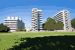
\includegraphics[height=0.3\textheight]{{figures/kit-demo/image-segmentation-h=0.1-K=gaussian}.png} &   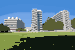
\includegraphics[height=0.3\textheight]{{figures/kit-demo/image-segmentation-h=0.2-K=gaussian}.png} \\
		(a) $h = 0.1$ & (b) $h = 0.2$ \\[6pt]
		
\includegraphics[height=0.3\textheight]{{figures/kit-demo/image-segmentation-h=0.3-K=gaussian}.png} &   
\includegraphics[height=0.3\textheight]{{figures/kit-demo/image-segmentation-h=0.4-K=gaussian}.png} \\
		(c) $h = 0.3$ & (d) $h = 0.4$ \\[6pt]
	\end{tabular}
	\caption{caption}
\end{figure}
\end{frame}


\begin{frame}{Image segmentation -- Gaussian kernel}
\tiny
\begin{figure}
\begin{tabular}{cc}
	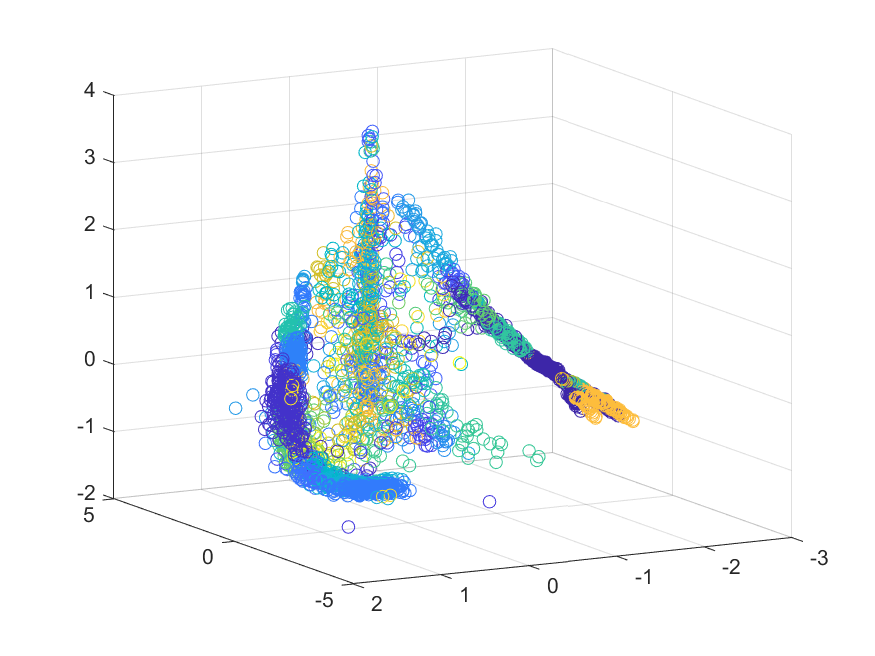
\includegraphics[height=0.3\textheight]{{figures/kit-demo/scatter-plot-h=0.1-K=gaussian}.png} &   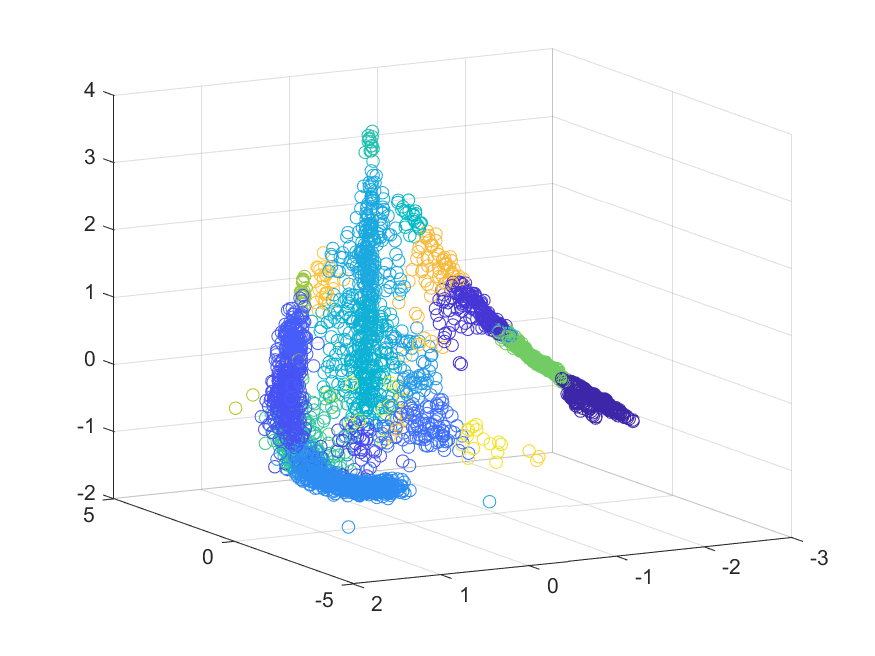
\includegraphics[height=0.3\textheight]{{figures/kit-demo/scatter-plot-h=0.2-K=gaussian}.png} \\
	(a) $h = 0.1$ & (b) $h = 0.2$ \\[6pt]
	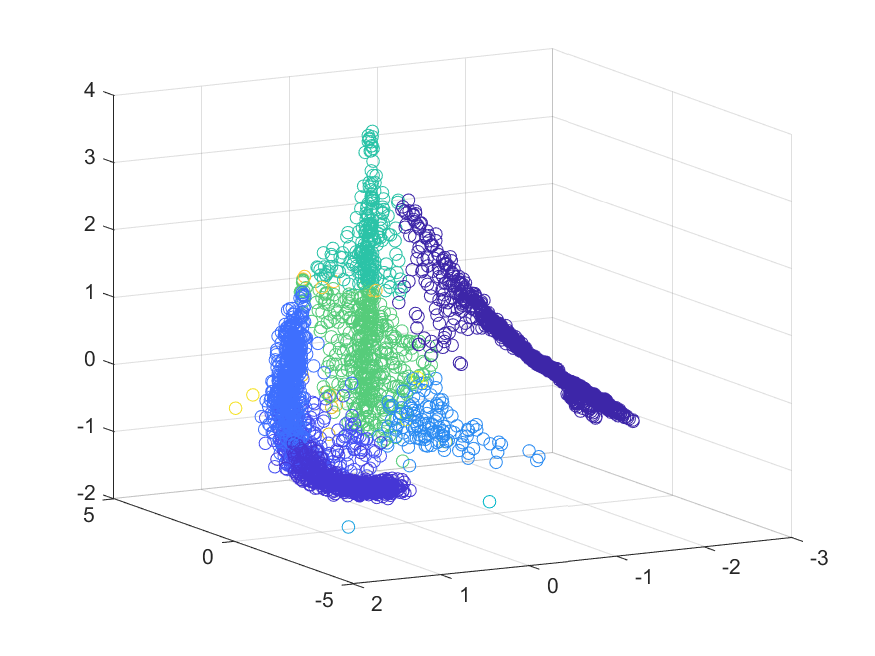
\includegraphics[height=0.3\textheight]{{figures/kit-demo/scatter-plot-h=0.3-K=gaussian}.png} &   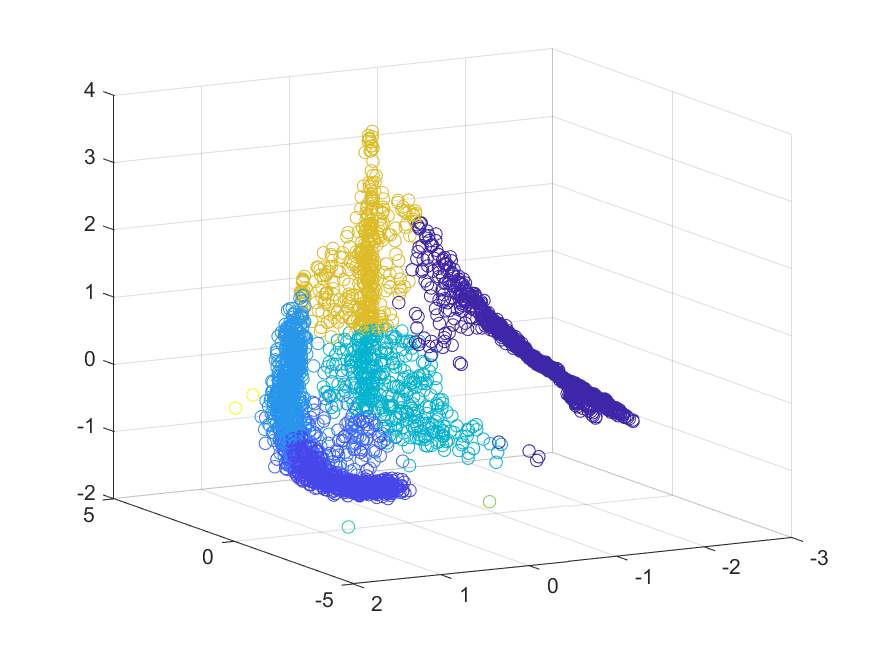
\includegraphics[height=0.3\textheight]{{figures/kit-demo/scatter-plot-h=0.4-K=gaussian}.png} \\
	(c) $h = 0.3$ & (d) $h = 0.4$ \\[6pt]
\end{tabular}
\caption{caption}
\end{figure}
\end{frame}


\begin{frame}{Image segmentation -- Uniform kernel}
\tiny
\begin{figure}
\begin{tabular}{cc}
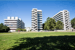
\includegraphics[width=0.4\textwidth]{{figures/kit-demo/image-segmentation-h=0.1-K=uniform}.png} &   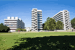
\includegraphics[width=0.4\textwidth]{{figures/kit-demo/image-segmentation-h=0.2-K=uniform}.png} \\
(a) $h = 0.1$ & (b) $h = 0.2$ \\[6pt]
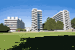
\includegraphics[width=0.4\textwidth]{{figures/kit-demo/image-segmentation-h=0.3-K=uniform}.png} &   
\includegraphics[width=0.4\textwidth]{{figures/kit-demo/image-segmentation-h=0.4-K=uniform}.png} \\
(c) $h = 0.3$ & (d) $h = 0.4$ \\[6pt]
\end{tabular}
\caption{caption}
\end{figure}
\end{frame}


\begin{frame}{Image segmentation -- Uniform kernel}
\tiny
\begin{figure}
\begin{tabular}{cc}
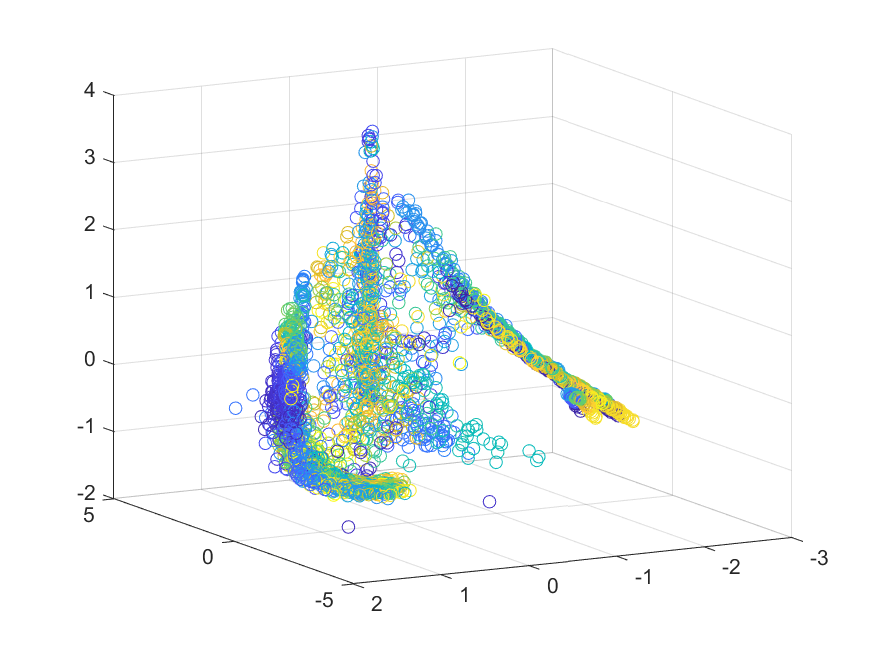
\includegraphics[height=0.3\textheight]{{figures/kit-demo/scatter-plot-h=0.1-K=uniform}.png} &   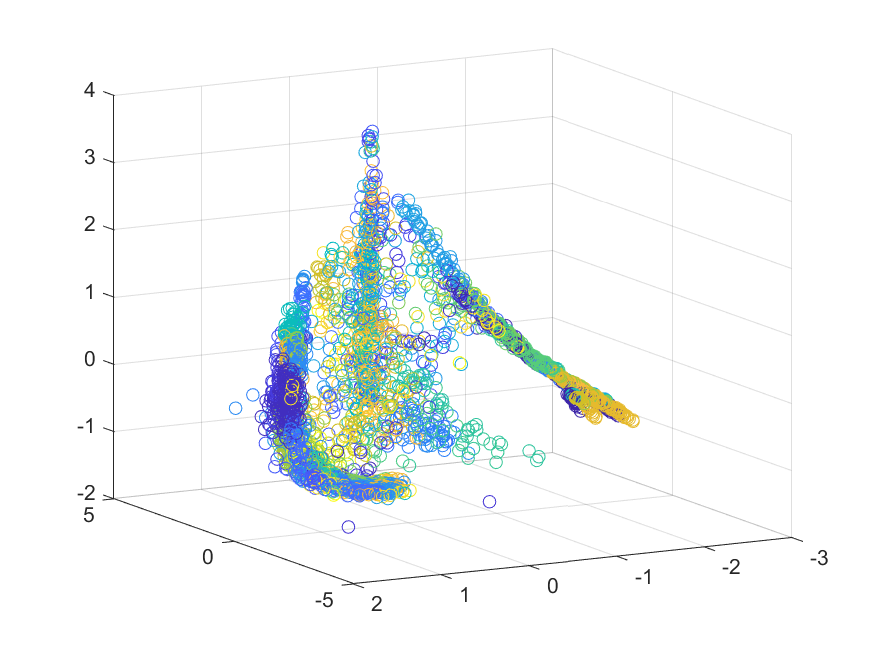
\includegraphics[height=0.3\textheight]{{figures/kit-demo/scatter-plot-h=0.2-K=uniform}.png} \\
(a) $h = 0.1$ & (b) $h = 0.2$ \\[6pt]
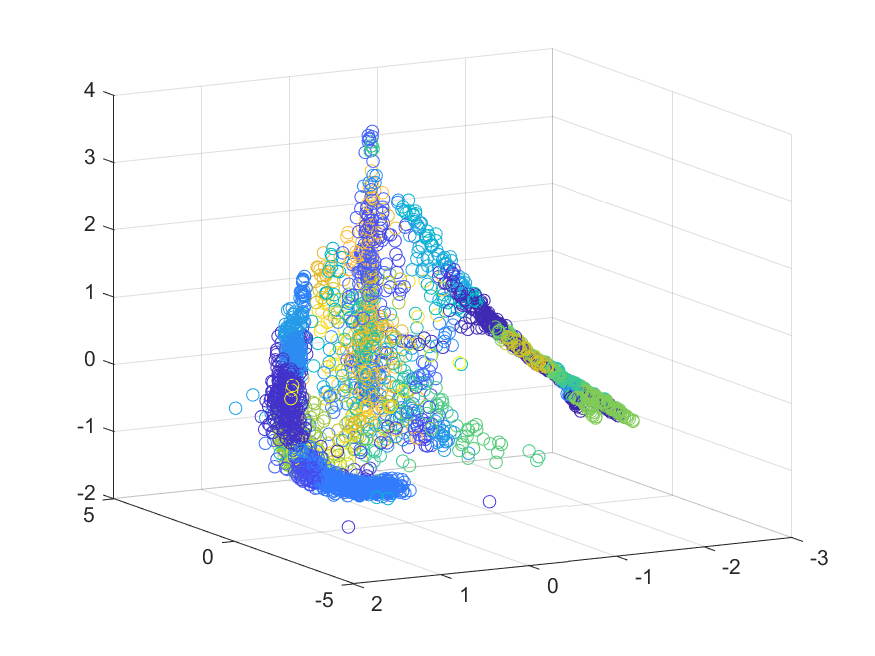
\includegraphics[height=0.3\textheight]{{figures/kit-demo/scatter-plot-h=0.3-K=uniform}.png} &   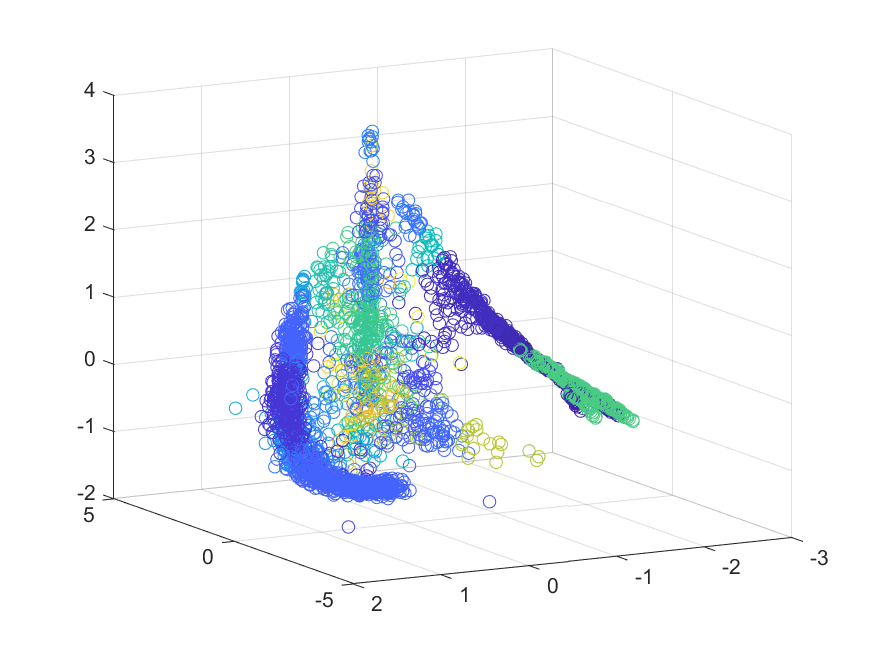
\includegraphics[height=0.3\textheight]{{figures/kit-demo/scatter-plot-h=0.4-K=uniform}.png} \\
(c) $h = 0.3$ & (d) $h = 0.4$ \\[6pt]
\end{tabular}
\caption{caption}
\end{figure}
\end{frame}


%\section{Section 1}
%\subsection{Subsection 1.1}
%\begin{frame}{Example slide A}
%	\begin{itemize}
%	\item PCM, Citation: \cite{becker2008a} %\language
%	\pause
%	\item Bullet point 2
%	\item \dots
%	\end{itemize}
%\end{frame}
%
%\subsection{TikZ}
%\begin{frame}{TikZ example}
%	\begin{tikzpicture}[level distance=10mm]
%	\tikzstyle{every node}=[fill=red!60,circle,inner sep=1pt]
%	\tikzstyle{level 1}=[sibling distance=20mm,
%	set style={{every node}+=[fill=red!45]}]
%	\tikzstyle{level 2}=[sibling distance=10mm,
%	set style={{every node}+=[fill=red!30]}]
%	\tikzstyle{level 3}=[sibling distance=5mm,
%	set style={{every node}+=[fill=red!15]}]
%	\node {31}
%	child {node {30}
%		child {node {20}
%			child {node {5}}
%			child {node {4}}
%		}
%		child {node {10}
%			child {node {9}}
%			child {node {1}}
%		}
%	}
%	child {node {20}
%		child {node {19}
%			child {node {1}}
%			child[fill=none] {edge from parent[draw=none]}
%		}
%		child {node {18}}
%	};
%	\end{tikzpicture}
%\end{frame}
%
%\subsection{Subsection 1.2}
%\begin{frame}{Example slide B}
%	\begin{block}{Block 1}
%	\begin{itemize}
%	\item Bullet point 1 $x \in X$
%	\pause
%	\item Bullet point 2
%	\item \dots
%	\end{itemize}
%	\end{block}
%\end{frame}
%
%\section{Section 2}
%\begin{frame}{Example slide C}
%	\begin{exampleblock}{Example 1}
%	\begin{itemize}
%	\item Bullet point 1
%	\pause
%	\item Bullet point 2
%	\item \dots
%	\end{itemize}
%	\end{exampleblock}
%\end{frame}
%
%\begin{frame}{Example slide D}
%	\begin{alertblock}{Alert 1}
%	\begin{itemize}
%	\item Bullet point 1
%	\pause
%	\item Bullet point 2
%	\item \dots
%	\end{itemize}
%	\end{alertblock}
%\end{frame}
%
%
%
%\section{Suchen und Sortieren}
%\subsection{Insertionsort}
%\begin{frame}
%\begin{algorithm}[H]
%	\caption{Euclid’s algorithm}\label{euclid}
%	\begin{algorithmic}[1]
%		\Procedure{Euclid}{$a,b$}\Comment{The g.c.d. of a and b}
%		\State $r\gets a\bmod b$
%		\While{$r\not=0$}\Comment{We have the answer if r is 0}
%		\State $a\gets b$
%		\State $b\gets r$
%		\State $r\gets a\bmod b$
%		\EndWhile\label{euclidendwhile}
%		\State \textbf{return} $b$\Comment{The gcd is b}
%		\EndProcedure
%	\end{algorithmic}
%\end{algorithm}
%\end{frame}


\appendix
\beginbackup

\begin{frame}[allowframebreaks]{References}
	%\printbibliography
	
	\bibliographystyle{agsm}
	\bibliography{../latex/KDEaMSC}
\end{frame}

\backupend

\end{document}
